% Created 2023-04-29 Sat 11:40
% Intended LaTeX compiler: pdflatex
\documentclass[11pt]{article}
\usepackage[utf8]{inputenc}
\usepackage[T1]{fontenc}
\usepackage{graphicx}
\usepackage{longtable}
\usepackage{wrapfig}
\usepackage{rotating}
\usepackage[normalem]{ulem}
\usepackage{amsmath}
\usepackage{amssymb}
\usepackage{capt-of}
\usepackage{hyperref}
\author{Yusheng Zhao}
\date{\today}
\title{Assignment 3}
\hypersetup{
 pdfauthor={Yusheng Zhao},
 pdftitle={Assignment 3},
 pdfkeywords={},
 pdfsubject={},
 pdfcreator={Emacs 28.2 (Org mode 9.6.1)}, 
 pdflang={English}}
\begin{document}

\maketitle


\section{Problem 1}
\label{sec:org65b8fcd}
From statistical mechanics, we know the following rule. When there is a phase
change, some function related to the structure of the system will change
abruptly. More specifically, you could calculate \textbf{RMSD} for the system under
investigation. Over time, you should see a discontinuity in the plot of time
versus \textbf{RMSD}. That's when a phase change occurred.

A plot may look something like this.

\begin{center}
\includegraphics[width=.9\linewidth]{../../../notes/imgs/pdfs/Problem_1/20230429-112158_Screenshot 2023-04-29 at 11.21.55.png}
\end{center}

\section{Problem 2}
\label{sec:org33cb368}
In a folded protein, I expect to find hydrophobic amino acids in the \textbf{innerds}
of the structure. Conversely, I expect to find hydrophilic amino acids on the
\textbf{outside} of the folded protein. This is basically due to the need to minimize
energy in the folded state of a protein.

\begin{itemize}
\item Hydrophobic Amino Acid: Alanine
\item Hydrophilic Amino Acid: Aspartic Acid
\item I have illustrated the protein: BARNASE MUTANT WITH ILE 88 REPLACED BY ALA
(1BRJ). In addition, I illustrated the hydrophobic amino acid, Alanine, as
balls. I also illustrated the hydrophilic amino acid, Aspartic Acid, as
surface.
\end{itemize}

\begin{center}
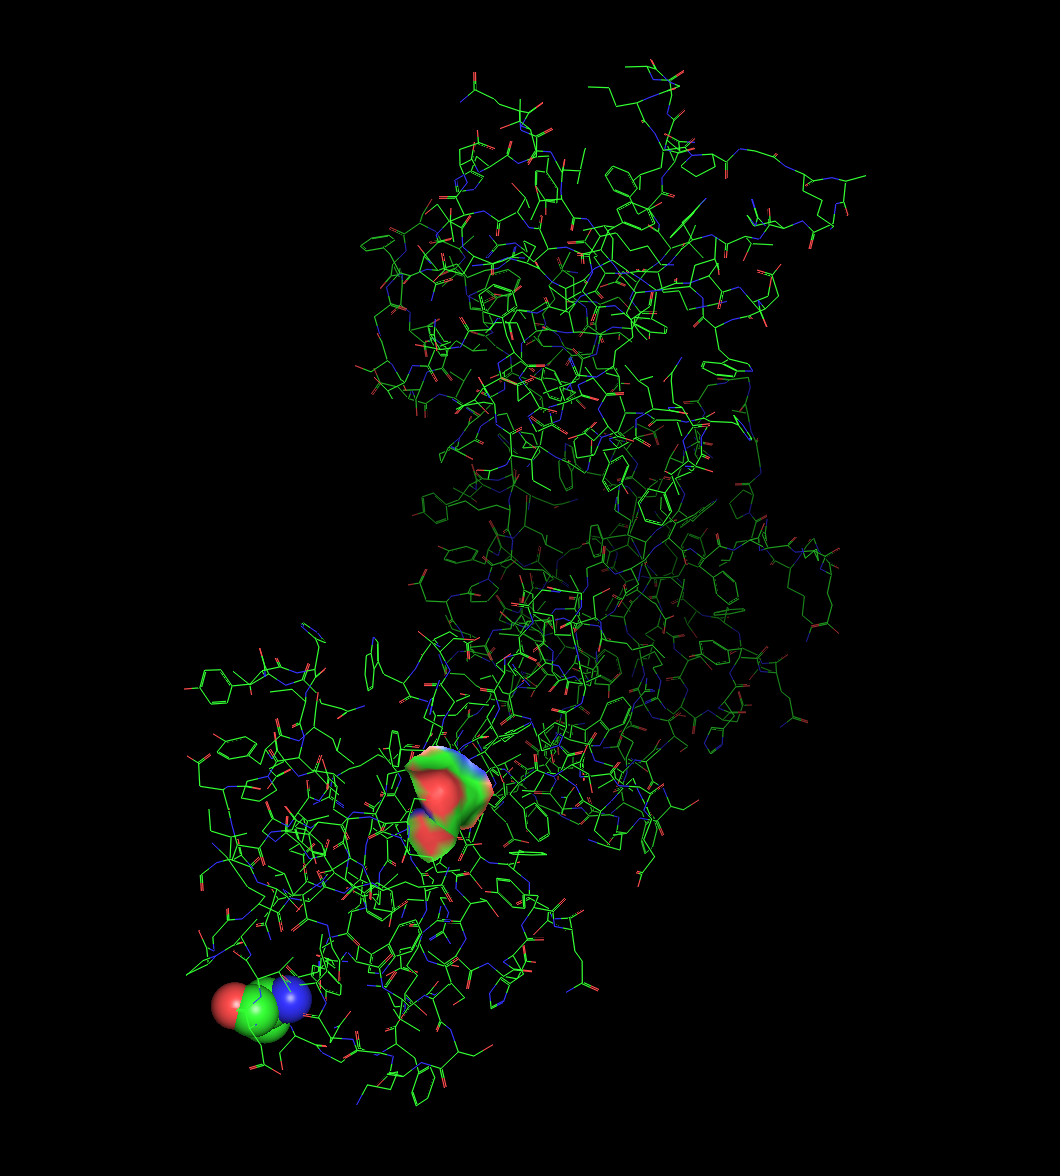
\includegraphics[width=.9\linewidth]{./protein.png}
\end{center}

\section{Problem 3}
\label{sec:orge1d5933}


\section{Problem 4}
\label{sec:orgeb77df6}
\end{document}